
BASELINES: BETA OG Z0 såvel som simons arbejde!!! Average intensity of all dyads. 

\subsection{First Research Question}
\label{sec:ResearchQuestion1}
The first research question of this project states:
\\
"How  well  can  dynamic  networks  be  modelled  using  a  SCVM  representation  in latent Euclidean space, with stepwise event computation?"
\\\\
In order to answer this question, the modelling approach will be evaluated on synthetically generated data.
Here synthetic dataset 1 is utilized, which is synthesized using a single velocity vector, as explained in section \ref{sec:Data:SyntheticData:SyntheticDataset1}.

\subsubsection{Modelling of single-step synthetic data}
\label{sec:ResearchQuestion1:singleStepSynthetic}
The first part of answering research question one consists of confirming proper modelling performance of a single-step Constant Velocity Model(CVM). 
This is done as an initial procedure as it lays the foundation of the stepwise CVM, meaning if the single-step model does not work as intended, the stepwise will neither.
\\\\
\textbf{Loss and beta convergence results.}
The stepwise model has been trained for 50, 500 and 5000 epochs on the full dataset 1 as one training batch using a single velocity step and a learning rate of 0.025. The model is compared against a baseline model which is simply a model with no dynamics i.e. a model with no velocities. Also for comparison the ground truth is provided.
Below, table \ref{tab:SingleStep1}, shows the learned beta parameter and final negative log loss, including that of the ground truth model.

\begin{table}[H]
\centering
\begin{tabular}{|l|c|cc|}
\hline
Model         & \multicolumn{1}{l|}{Num. Epochs} & Beta & Avg. NLL \\ \hline
Ground Truth  & -                                & 7.5  & -82,000  \\
No V Baseline & 5000                             & XX   & XX       \\
1 Step Model  & 5                                & XX   & XX       \\
1 Step Model  & 5000                             & XX   & XX       \\ \hline
\end{tabular}
\caption{Final learned $\beta$ value and negative log loss for baseline trained model.}
\label{tab:SingleStep1}
\end{table}

\\\\
\textbf{Intensity rate comparison results.}
\\
The intensity rates for a 5000 epochs trained model on 

\begin{figure}[H]
    \centering
    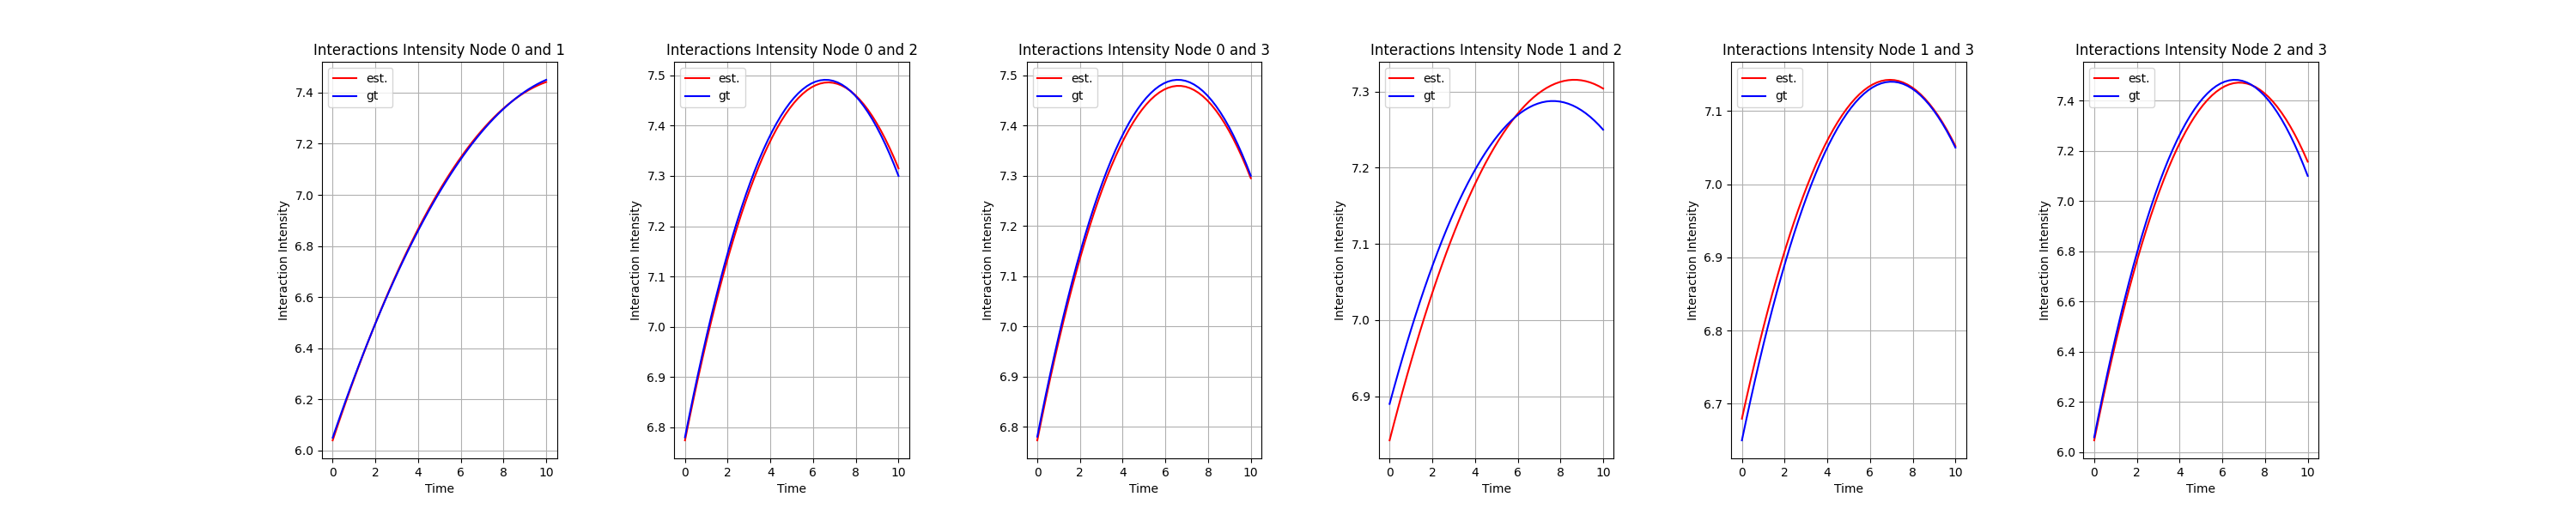
\includegraphics[width=\textwidth]{0_images/synth1_epochs5000.png}
    \caption{Node pair interaction intensity for synthetic dataset 1 trained for 5000 epochs. Blue line is the ground truth model, red is the trained model.}
    \label{fig:RQ1synth1}
\end{figure}
\\\\
\textbf{Animation check.}
\\\\
\textbf{Interaction removal results.}
The results from interaction removal, as explained in \ref{sec:Method:Evaluation:AUC}, shows quite a bad 
\\\\
\textbf{Dyad removal results.}

The baseline that has no dynamics is killed here, as it is not even able to be intepreted for intensity rate comparison.




\subsubsection{Multi-step TDGN modelling of synthetic data}
\label{sec:ResearchQuestion1:multiStepSynthetic}
The second part of answering the first research question evaluates the SCVM with 10 steps to test its capabilities with multiple steps.
The test uses the synthetic dataset 2, see section \ref{sec:Data:SyntheticData:SyntheticDataset2}.
\\\\
\textbf{Loss and beta convergence results.}

\begin{table}[H]
\centering
\begin{tabular}{|l|cc|}
\hline
Num. Epochs   & Beta & NLL\\ \hline
Ground Truth & 7.5  & -6.29      \\
5          & XX   & XX       \\
50          & 7.438   & -6.208       \\
500          & XX   & XX       \\
2500          & XX   & XX       \\
5000          & XX   & XX       \\
\hline
\end{tabular}
\caption{Final learned $\beta$ value and negative log loss for trained model on synthetic dataset 2 \ref{sec:Method:Reproducibility:SyntheticDataset2}}
\label{tab:MultiStep1}
\end{table}

\noindent \textbf{Intensity rate comparison results.}
\\\\
\textbf{Animation check.}
\\\\
\textbf{Interaction removal results.}
The 
\\\\
\textbf{Dyad removal results.}



\subsubsection{Multi-step modelling of real world data}
\label{sec:ResearchQuestion1:ResistanceTraining}
The third part of answering the first research question investigates the SCVM's modelling capabilities on a real world dataset.
\\
Real dataset 1, see section \ref{sec:Data:RealData:RealDataset1}, is utilized here.
\\\\
\textbf{Animation check.}
\\\\
\textbf{Interaction removal results.}



